\chapter{App. methods: perturbation theory}
The perturbation analysis depends strongly on the problem: we distinguish stationary ($\partial_tH = 0$) from non-stationary ($\partial_tH \neq 0$) problems and concentrate on discrete spectra. In the simplest case there is a non-degenerate spectrum - we therefore treat the stationary, non-degenerate case first and then analyze degenerate and almost degenerate eigenvalues. Non-stationary problems and Fermi's Golden Rule conclude the discussion.

\section{Stationary, non-degenerate case}
Given the stationary ($\partial_tH = 0$) eigenvalue problem
%公式 1
\begin{equation}
    H\Psi=E\Psi
\end{equation}
The Hamiltonian decay into $H = H_0 + H'$, with $H_0$ simple enough to be a solution
%公式 2
\begin{equation}
\begin{array}{c}{H_{0} \varphi_{n}=\mathcal{E}_{n} \varphi_{n}} \\ {\varphi_{n} \text { ein vONS }} \\ {\operatorname{dim} \operatorname{Eig} \mathcal{E}_{n}=1}\end{array}
\end{equation}
is known. $H'$ is a small disturbance; we are looking for a series of disturbances in $H'$. We write to make the bookkeeping easier
%公式 3
\begin{equation}
    H=H_0+\lambda H'
\end{equation}
and apply a perturbation approach in $\lambda$,
%公式 4
\begin{equation}
\begin{array}{l}{\Psi=\Psi_{0}+\lambda \Psi_{1}+\lambda^{2} \Psi_{2}+\lambda^{3} \Psi_{3}+\cdots} \\ {E=E_{0}+\lambda E_{1}+\lambda^{2} E_{2}+\lambda^{3} E_{3}+\cdots}\end{array}
\end{equation}
Inserting (9.4) in (9.1) with (9.3) results in OK
%公式 5
\begin{equation}
\begin{array}{ccll} 
\lambda^{0}: \qquad&\left(H_{0}-E_{0}\right) &\Psi_{0}=0 \\ 
\lambda^{1}: \qquad&\left(H_{0}-E_{0}\right) &\Psi_{1}=\left(E_{1}-H^{\prime}\right) \Psi_{0} \\ 
\lambda^{2}: \qquad&\left(H_{0}-E_{0}\right) &\Psi_{2}=\left(E_{1}-H^{\prime}\right) \Psi_{1}+E_{2} \Psi_{0} \\ 
\lambda^{3}: \qquad&\left(H_{0}-E_{0}\right) &\Psi_{3}=\left(E_{1}-H^{\prime}\right) \Psi_{2}+E_{2} \Psi_{1}+&E_{3} \Psi_{0} \\ 
& &\;\uparrow  \qquad\qquad\qquad\qquad &\uparrow \\ 
& \qquad \text { hochstes } &\Psi_{n} &\text { hochstes } E_n
\end{array}
\end{equation}
The order $\lambda^0$ immediately shows that
%公式 6
\begin{equation}
    \Psi_0 = \varphi_n,\qquad E_0=\varepsilon_n.
\end{equation}
Further, we can find the $\Psi_k$ iteratively because only $\Psi_j$ with $j <k$ appear to the right of the equals signs. The addition of $\mu_k\Psi_0$ to $\Psi_k$, $\Psi_k$ $\rightarrow$ $\Psi_k+\mu_k \Psi_0$  does not change the equation for $\Psi_k$, since
%公式 7
\begin{equation}
    \left(H_{0}-E_{0}\right) \mu_{k} \Psi_{0}=\mu_{k}\left(H_{0}-\mathcal{E}_{n}\right) \varphi_{n}=\mu_{k}\left(\mathcal{E}_{n}-\mathcal{E}_{n}\right) \varphi_{n}=0
    \end{equation}
Without limiting the generality, we can therefore count and demand from $\Psi_k$ its component along $\Psi_0$
%公式 8
\begin{equation}
    \langle\Psi_0|\Psi_k\rangle =\delta_{0k},
\end{equation}
what a standardization condition
%公式 9
\begin{equation}
    \langle\varphi_n|\Psi\rangle = 1
\end{equation}
equals. We want to solve (9.5) systematically. The scalar product with $\Psi_0$ gives the order $\lambda$s equation
%公式 10

\begin{align} \underbrace{\left\langle\Psi_{0}\left|H_{0}-E_{0}\right| \Psi_{s}\right\rangle} &=\underbrace{\left\langle\Psi_{0}\left|E_{1}-H^{\prime}\right| \Psi_{s-1}\right\rangle}_{\delta_{s 1} E_{1}-\left\langle\Psi_{0}\left|H^{\prime}\right| \Psi_{s-1}\right\rangle}+\sum_{j=2}^{s} E_{j} \underbrace{\left\langle\Psi_{0} | \Psi_{s-j}\right\rangle}_{\delta_{s j}} \\ 
 \Rightarrow E_{s} &=\left\langle\varphi_{n}\left|H^{\prime}\right| \Psi_{s-1}\right\rangle, \quad s \geq 1 \end{align}

%公式 11
the calculation of $E$ in order s presupposes the calculation of $\Psi$ in the order $s - 1$.

We find an interesting intermediate result by multiplying (9.11) by $\lambda^s$ and then summing over all orders ¨ $\lambda^s$; this manipulation gives a relationship between $E$ and $\Psi$ in the form

%公式 12
\begin{equation}
    E=\mathcal{E}_{n}+\lambda\left\langle\varphi_{n}\left|H^{\prime}\right| \Psi\right\rangle
    \end{equation}
For a systematic calculation of ¨ $E$ and $\Psi$ we need an expression for ¨ $|\Psi_s\rangle$ and we develop in the basis $|\varphi_l\rangle$,
%公式 13
\begin{equation}
    \left|\Psi_{s}\right\rangle=\sum_{l}^{\prime}\left\langle\varphi_{l} | \Psi_{s}\right\rangle\left|\varphi_{l}\right\rangle, \quad s \geq 1
    \end{equation}
The sum $\sum'$ contains no term $l = n$ since $\langle\varphi_n|\Psi_s\rangle=\langle\Psi_0|\Psi_s\rangle=\delta_{0s}$, cf. Eq. (9.8). The scalar product of (9.5) in the order $s$ with $\langle\varphi_l|$ results
%公式 14
\begin{equation}
    \underbrace{\left\langle\varphi_{l}\left|H_{0}\right| \Psi_{s}\right\rangle}_{\varepsilon_{l}\left(\varphi_{l} | \Psi_{s}\right)}+\left\langle\varphi_{l}\left|H^{\prime}\right| \Psi_{s-1}\right\rangle=\sum_{j=0}^{s} E_{j}\left\langle\varphi_{l} | \Psi_{s-j}\right\rangle
    \end{equation}
where the term with $j = 0$ in total, $E_0\langle\varphi_l|\Psi_s\rangle$, again contains $|\Psi_s\rangle$. We find that
%公式 15
\begin{equation}
    \left\langle\varphi_{l} | \Psi_{s}\right\rangle=\frac{1}{\mathcal{E}_{n}-\mathcal{E}_{l}}\left[\left\langle\varphi_{l}\left|H^{\prime}\right| \Psi_{s-1}\right\rangle-\sum_{j=1}^{s} E_{j}\left\langle\varphi_{l} | \Psi_{s-j}\right\rangle\right]
    \end{equation}
This system of equations can be solved iteratively: Let $E$ and $\Psi$ be known up to and including the order $s - 1$, which means that $E_0, \cdots, E_{s − 1}$ and $\Psi_0$, $\cdots$, $\Psi_{s-1}$ have already been found. Then for ¨ $s\geq 1$:
%公式 16
\begin{equation}
\begin{array}{ll}\,{(9.11) \quad E_{s} =\left\langle\varphi_{n}\left|H^{\prime}\right| \Psi_{s-1}\right\rangle \text { and }} \\ 
{\left.\begin{array}{c}
    {(9.13)}\\{(9.15)}
\end{array}\right\}
  \left|\Psi_{s}\right\rangle=\sum_{l \neq n} \frac{\left\langle\varphi_{l}\left|H^{\prime}\right| \Psi_{s-1}\right\rangle-\sum_{j=1}^{s} E_{j}\left\langle\varphi_{l} | \Psi_{s-j}\right\rangle}{\mathcal{E}_{n}-\mathcal{E}_{l}}\left|\varphi_{l}\right\rangle}\end{array}
\end{equation}
For ¨ $s = 0, E_0 = \varepsilon_n$ and $|\Psi_0\rangle$ = $|\varphi_n\rangle$ form the starting point for the iteration. The non-degeneracy was important in (9.15): There must be no vector $|\varphi_i\rangle\neq|\varphi_n\rangle$ with $\varepsilon_l = \varepsilon_n$. We will come back to the special case where this condition is not met. Finally, we explicitly state the results for ¨ $s \leq 2$, using the notation $|\varphi_l\rangle=|l\rangle$:
%公式 17
\begin{equation}
\lambda^{0}: \quad\left\{\begin{aligned} E_{0} &=\mathcal{E}_{n} \\\left|\Psi_{0}\right\rangle &=|n\rangle \end{aligned}\right.
\end{equation}
%公式 18
\begin{equation}
\lambda^{1}: \quad\left\{\begin{aligned} E_{1} &=\left\langle n\left|H^{\prime}\right| n\right\rangle \\\left|\Psi_{1}\right\rangle &=\sum_{l \neq n} \frac{\left\langle l\left|H^{\prime}\right| n\right\rangle}{\varepsilon_{n}-\mathcal{E}_{l}}|l\rangle \end{aligned}\right.
\end{equation}
%公式 19
\begin{equation}
\lambda^{2}:\left\{\begin{aligned} E_{2} &=\quad \sum_{l \neq n} \frac{\left|\left\langle l\left|H^{\prime}\right| n\right\rangle\right|^{2}}{\mathcal{E}_{n}-\mathcal{E}_{l}} \\\left|\Psi_{2}\right\rangle &=\sum_{l \neq n}\left[\sum_{k \neq n} \frac{\left\langle l\left|H^{\prime}\right| k\right\rangle\left\langle k\left|H^{\prime}\right| n\right\rangle}{\left(\mathcal{E}_{n}-\mathcal{E}_{l}\right)\left(\mathcal{E}_{n}-\mathcal{E}_{k}\right)}-\frac{\left\langle l\left|H^{\prime}\right| n\right\rangle\left\langle n\left|H^{\prime}\right| n\right\rangle}{\left(\mathcal{E}_{n}-\mathcal{E}_{l}\right)^{2}}\right]|l\rangle \end{aligned}\right.
\end{equation}
The normalization (in order $s = 2$) has the form
%公式 20
\begin{equation}
    \langle\Psi | \Psi\rangle= 1+\sum_{l \neq n} \frac{\left|\left\langle l\left|H^{\prime}\right| n\right\rangle\right|^{2}}{\left(\mathcal{E}_{n}-\mathcal{E}_{l}\right)^{2}}
    \end{equation}
Note: The 2nd order of perturbation theory always leads to a lowering of the ground state energy.
Example: Harmonic oscillator in the force field The problem is caused by the Hamiltonian
%公式 21
\begin{equation}
\begin{aligned} H &=H_{0}+H^{\prime} \\ H_{0} &=\frac{p^{2}}{2 m}+\frac{1}{2} m \omega^{2} q^{2}, \quad \omega^{2}=f / m \\ H^{\prime} &=-F q \end{aligned}
\end{equation}
Are defined. The undisturbed problem has the solution
%公式 22
\begin{equation}
\begin{aligned} H_{0}|n\rangle &=\mathcal{E}_{n}|n\rangle \\ \mathcal{E}_{n} &=\hbar \omega(n+1 / 2) \end{aligned}
\end{equation}
We go to dimensionless variables and introduce ascent and descent operators (see page 110 ff)
%公式 23
\begin{equation}
    q=\sqrt{\frac{\hbar}{m \omega}} x=\sqrt{\frac{\hbar}{2 m \omega}}\left(a+a^{\dagger}\right)
    \end{equation}
The matrix elements result in
%公式 24
\begin{equation}
\begin{aligned}\left\langle k\left|H^{\prime}\right| l\right\rangle &=- F \sqrt{\frac{\hbar l}{2 m \omega}}\langle k | l-1\rangle- F \sqrt{\frac{\hbar(l+1)}{2 m \omega}}\langle k | l+1\rangle \\ &=- F \sqrt{\frac{\hbar l}{2 m \omega}} \delta_{k, l-1}-F \sqrt{\frac{\hbar(l+1)}{2 m \omega}} \delta_{k, l+1} \end{aligned}
\end{equation}
This gives us the following results up to the 2nd order,\footnote{1The components $|\Psi_i\rangle$ listed here result in the normalized wave function; if one follows the above scheme, the terms $|\Psi_{i\geq 1}\rangle$ are orthogonalized to $|\Psi_0\rangle$ and then normalized. The comparison with the exact result then involves a development of the standardization factor}
%公式 25
\begin{equation}
\begin{array}{ll} 
0^{\mathrm{te}}: & E_{0}=\left(n+\frac{1}{2}\right)\hbar \omega \\
\left|\Psi_{0}\right\rangle &=|n\rangle \end{array}
\end{equation}
%公式 26
\begin{equation}
\begin{aligned} 1^{\text {te }}: &=\left\langle n\left|H^{\prime}\right| n\right\rangle= 0 \\\left|\Psi_{1}\right\rangle &=\sum_{l \neq n} \frac{\left\langle l\left|H^{\prime}\right| n\right\rangle}{\mathcal{E}_{n}-\mathcal{E}_{l}}|l\rangle \\ &=-\frac{F \sqrt{m \hbar \omega / 2}}{m \hbar \omega^{2}}(-\sqrt{n+1}|n+1\rangle+\sqrt{n}|n-1\rangle) \\ &=\frac{-i F}{m \hbar \omega^{2}} p|n\rangle \quad \text { mit } \quad p=\sqrt{\frac{m \hbar \omega}{2}} \frac{1}{i}\left(a-a^{\dagger}\right) \end{aligned}
\end{equation}
%
\begin{equation}
\begin{aligned} 2^{\text {te }}: &=\sum_{l \neq n} \frac{\left|\left\langle l\left|H^{\prime}\right| n\right\rangle\right|^{2}}{\mathcal{E}_{n}-\mathcal{E}_{l}} \\ &=\frac{\left|\left\langle n\left|H^{\prime}\right| n+1\right\rangle\right|^{2}}{-\hbar \omega}+\frac{\left|\left\langle n\left|H^{\prime}\right| n-1\right\rangle\right|^{2}}{\hbar \omega}=-\frac{F^{2}}{2 m \omega^{2}} \\\left|\Psi_{2}\right\rangle_{\text {Normiert }} &=-\frac{1}{2}\left(\frac{F}{m \hbar \omega^{2}}\right)^{2} p^{2}|n\rangle \end{aligned}
\end{equation}
On the other hand, Hamiltonia describes
%公式
$$
\begin{aligned} H &=\frac{p^{2}}{2 m}+\frac{1}{2} m \omega^{2} q^{2}-F q \\ &=\frac{p^{2}}{2 m}+\frac{m \omega^{2}}{2}(q-\underbrace{\frac{F}{m \omega^{2}}}_{q_{0}})^{2} \underbrace{-\frac{F^{2}}{2 m \omega^{2}}}_{E_{2}} \end{aligned}
$$
just a harmonic oscillator shifted by $q_0 = F / mw^2$; whose energies are shifted by $-F^2 / 2mw^2$
%公式 28
\begin{equation}
    E=\left(n+\frac{1}{2}\right) \hbar \omega-\frac{F^{2}}{2 m \omega^{2}}
    \end{equation}
and the state functions sin
%公式 29
\begin{equation}
\begin{aligned}|\Psi\rangle &=\exp \left[-i p q_{0} / \hbar\right]|n\rangle=\exp \left[-i p F / m \hbar \omega^{2}\right]|n\rangle \\ & \cong|n\rangle-\frac{i p F}{m \hbar \omega^{2}}|n\rangle-\frac{1}{2}\left(\frac{F p}{m \hbar \omega^{2}}\right)^{2}|n\rangle \end{aligned}
\end{equation}
The perturbation series should just result in the shifted harmonic oscillator as a power series in $F$, which is confirmed by the comparison of (9.25) - (9.27) with (9.28) and (9.29).

\section{Stationary, degenerate case}
The problem of degeneracy is expressed in (9.15) - the energy denominator $\varepsilon_n-\varepsilon_l$ disappears if $| n\rangle$ and $| l\rangle$ come from the same energy space and therefore have the same energy. Remedy is simple: we have to rebuild the perturbation theory for degenerate eigenvalues. Note that degeneration is only relevant if we carry out the perturbation analysis in the degenerate eigenspace, but not if we have dim Eig ¨ $\varepsilon_m = D_m> 1$ but examine Eigen $\varepsilon_{n|\varepsilon_n\neq\varepsilon_m}$ with dim Eig $\varepsilon_n = 1$. In the latter case, all denominators En - Em are constant over Eig ¨ $\varepsilon_m$, but $\varepsilon_n-\varepsilon_n\neq 0$.

We work out a concrete example with dim Eig $\varepsilon_m = 2$, the general case with dim Eig $\varepsilon_m = k> 1$ follows trivially; instead of a $2 \times 2$ matrix, a $k \times k$ matrix is ​​to be diagonalized, see later. Let $\{\varphi_m,\varphi_n\}$ be the eigenspace for $E_0=\varepsilon_m=\varepsilon_n=\varepsilon$ and $\varphi_n\perp\varphi_m$.

\subsection{Abolition of the degeneracy in the order $s = 1$}
The energy alone is not enough to determine the state to be examined since all superpositions
%公式 30
\begin{equation}
    \Psi_0 = a_m|m\rangle+a_n|n\rangle
\end{equation}
have the same energy $E_0 = \varepsilon$ okay $s = 0$ (we use the Diracnotation $\varphi_l\rightarrow|l\rangle$. We can find a good starting point for the series of perturbations if we take (9.5) $s = 1$ and matrix elements with $\langle m|$ and $\langle n|$ form,

%公式 31
\begin{equation}
\begin{aligned} \underbrace{\left\langle m\left|H_{0}-E_{0}\right| \Psi_{1}\right\rangle}_{0}=\left\langle m\left|E_{1}-H^{\prime}\right| \Psi_{0}\right\rangle \\= a_{m}\left\langle m\left|E_{1}\right| m\right\rangle+ a_{n} \underbrace{\left\langle m\left|E_{1}\right| n\right\rangle}_{0} \\-a_{m}\left\langle m\left|H^{\prime}\right| m\right\rangle- a_{n}\left\langle m\left|H^{\prime}\right| n\right\rangle \end{aligned}
\end{equation}
and also with $\langle n |$. The two equations can be put into the following matrix form,
%公式 32
\begin{equation}
    \begin{array}{ccc}
        \left(\left\langle m\left|H^{\prime}\right| m\right\rangle- E_{1}\right) a_{m}&+&\left\langle m\left|H^{\prime}\right| n\right\rangle a_{n}=0\\
        \left\langle n\left|H^{\prime}\right| m\right\rangle a_{m}&+&\left(\left\langle n\left|H^{\prime}\right| n\right\rangle- E_{1}\right) a_{n}=0
    \end{array}
    \end{equation}
With $\langle m|H'|m\rangle\equiv\varepsilon'_m$ and $\langle n|H'|n\rangle\equiv\varepsilon'_n$ sucha as $\langle m|H'|n\rangle=\langle n|H'|m\rangle^*\equiv\delta'$ we get the eigenvalue problem
%公式 33
\begin{equation}
\left(\begin{array}{cc}{\mathcal{E}_{m}^{\prime}-E_{1}} & {\delta^{\prime}} \\ {\delta^{\prime *}} & {\mathcal{E}_{n}^{\prime}-E_{1}}\end{array}\right)\left(\begin{array}{c}{a_{m}} \\ {a_{n}}\end{array}\right)=0
\end{equation}
A solution $\Psi_0\neq 0$ exists if the determinant equals zero, that is
%公式 34
\begin{equation}
    \left(\mathcal{E}_{m}^{\prime}-E_{1}\right)\left(\mathcal{E}_{n}^{\prime}-E_{1}\right)-\left|\delta^{\prime}\right|^{2}=0
    \end{equation}
which allows us to calculate $E_1$
%公式 35
\begin{equation}
    E_{1}^{\pm}=\frac{\mathcal{E}_{m}^{\prime}+\mathcal{E}_{n}^{\prime}}{2} \pm \sqrt{\left(\frac{\mathcal{E}_{m}^{\prime}-\mathcal{E}_{n}^{\prime}}{2}\right)^{2}+\left|\delta^{\prime}\right|^{2}}
    \end{equation}
The conditions
%公式 36
\begin{equation}
\begin{aligned} \frac{a_{m}^{\pm}}{a_{n}^{\pm}} &=\frac{\delta^{\prime}}{E_{1}^{\pm}-\mathcal{E}_{m}^{\prime}} \\\left|a_{m}^{\pm}\right|^{2}+\left|a_{n}^{\pm}\right|^{2} &=1 \end{aligned}
\end{equation}
characterize the associated eigenvectors.

Let $\mathcal{E}'_m\neq\mathcal{E}'_n$ or $\delta'\neq 0$. In the lowest order we get the result $E_0 = \mathcal{E}$ and $| \Psi_0^{\pm}=a_m^{\pm}|m\rangle+a_n^{\pm}|n\rangle$ with $a_m^{\pm},a_n^{\pm}$ determined by (9.36). The next order gives the corrector $E_1 = E_1^{\pm}$ according to (9.35) and the degeneracy is canceled. To find the corrections | $\Psi$ ± 1i for the wave functions we first consider the order $s = 1$ of (9.5) and calculate the matrix element with $\langle l |, l \neq m, n,$
%公式 37
\begin{equation}
\begin{aligned}\left\langle l\left|H_{0}-E_{0}\right| \Psi_{1}^{\pm}\right\rangle &=\left\langle l\left|E_{1}^{\pm}-H^{\prime}\right| \Psi_{0}^{\pm}\right\rangle \\\left(\mathcal{E}_{l}-\mathcal{E}\right)\left\langle l | \Psi_{1}^{\pm}\right\rangle &= E_{1}^{\pm} \underbrace{\left\langle l | \Psi_{0}^{\pm}\right\rangle}_{0}-\left\langle l\left|H^{\prime}\right| \Psi_{0}^{\pm}\right\rangle \end{aligned}
\end{equation}
(9.37) defines the components of $|\Psi_1^{\pm}\rangle$  in the sector $\mathcal{H} \backslash \{| m\rangle, | n\rangle\}$,
%公式 38
\begin{equation}
    \left|P \Psi_{1}^{\pm}\right\rangle=\sum_{l \neq m, n} \frac{\left\langle l\left|H^{\prime}\right| \Psi_{0}^{\pm}\right\rangle}{\mathcal{E}-\mathcal{E}_{l}}|l\rangle
    \end{equation}
where the projector $P=\mathbb{I}-|m\rangle\langle m|-| n\rangle\langle n|$ projected on $\mathcal{H} \backslash\{|m\rangle,|n\rangle\}$. In addition, we also have to determine the components of ¨ $|\Psi_1^{\pm}\rangle$ in space $\{|m\rangle,|n\rangle\}$, for which we use the next order, the $\lambda^2$ term in (9.5). For ¨ $|\Psi_1^{\pm}\rangle$ we find
%公式 39
\begin{equation}
\begin{aligned}
\left\langle\Psi_{0}^{-}\left|\cdot\left(H_{0}-E_{0}\right)\right| \Psi_{2}^{+}\right\rangle=&\left(E_{1}^{+}-H^{\prime}\right)\left|\Psi_{1}^{+}\right\rangle+ E_{2}^{+}\left|\Psi_{0}^{+}\right\rangle \\ 
\underbrace{\left\langle\Psi_{0}^{-}\left|H_{0}-E_{0}\right| \Psi_{2}^{+}\right\rangle}_{0}=&\left\langle\Psi_{0}^{-}\left|E_{1}^{+}-H^{\prime}\right| \Psi_{1}^{+}\right\rangle+ E_{2}^{+} \underbrace{\left\langle\Psi_{0}^{-} | \Psi_{0}^{+}\right\rangle}_{0} \\ 
& \rightarrow\left\langle\Psi_{1}^{+}\left|E_{1}^{+}-H^{\prime}\right| \Psi_{0}^{-}\right\rangle= 0 \end{aligned}
\end{equation}
On the other hand
%公式 40
\begin{equation}
\begin{aligned}\left(E_{1}^{+}-H^{\prime}\right)\left|\Psi_{0}^{-}\right\rangle &=\left(E_{1}^{+}-P H^{\prime}\right)\left|\Psi_{0}^{-}\right\rangle-(11-P) H^{\prime}\left|\Psi_{0}^{-}\right\rangle \\ &=\left(E_{1}^{+}-E_{1}^{-}\right)\left|\Psi_{0}^{-}\right\rangle- P H^{\prime}\left|\Psi_{0}^{-}\right\rangle \end{aligned}
\end{equation}
da $(\mathbb{I}-P) H^{\prime}\left|\Psi_{0}^{-}\right\rangle= E_{1}^{-}\left|\Psi_{0}^{-}\right\rangle$ as shown by direct recalculation. The combination of (9.39) and (9.40) yields
%公式 41
\begin{equation}
    0=\left(E_{1}^{+}-E_{1}^{-}\right)\left\langle\Psi_{0}^{-} | \Psi_{1}^{+}\right\rangle-\left\langle\Psi_{0}^{-}\left|H^{\prime} P\right| \Psi_{1}^{+}\right\rangle
    \end{equation}
and thus, using (9.38), the component $\left\langle\Psi_{0}^{-} | \Psi_{1}^{+}\right\rangle$. Note that the correction (9.41) is of the order $\left\langle m(n)\left|H^{\prime}\right| l\right\rangle\left\langle l\left|H^{\prime}\right| m(n)\right\rangle\left(E_{1}^{+}-E_{1}^{-}\right)^{-1} \sim \mathcal{O}\left(H^{\prime}\right)$. An analogous calculation gives the corresponding result for ¨ $|\Psi_1^{-}\rangle$. If we summarize the above results, we find a series of problems starting with
%公式 42
\begin{equation}
\begin{array}{l}
{\left\{\begin{array} {ccl}
    E_{0} &=&\mathcal{E} ; \\
    \left|\Psi_{0}^{+}\right\rangle &=& a_{m}^{+}|m\rangle+ a_{n}^{+}|n\rangle ; \\
    \end{array}\right.}\qquad
    {\left\{\begin{array} {ccl}
        E_{0} &=&\mathcal{E} ; \\
        \left|\Psi_{0}^{-}\right\rangle &=& a_{m}^{-}|m\rangle+ a_{n}^{-}|n\rangle ; \\
        \end{array}\right.}\\\\    
{\left\{\begin{array}{ccl}
    E_{1} &=& E_{1}^{+} \\
    \left|\Psi_{1}^{+}\right\rangle &=&\sum_{l \neq m, n}\left[\frac{\left\langle\Psi_{0}^{-}\left|H^{\prime}\right| l\right\rangle\left(l\left|H^{\prime}\right| \Psi_{0}^{+}\right\rangle}{\left(E_{1}^{+}-E_{1}^{-}\right)\left(\mathcal{E}-\mathcal{E}_{l}\right)}\left|\Psi_{0}^{-}\right\rangle+\frac{\left\langle l\left|H^{\prime}\right| \Psi_{0}^{+}\right\rangle}{\mathcal{E}-\mathcal{E}_{l}}|l\rangle\right]
\end{array}\right.}\\\\
{\left\{\begin{array}{ccl}
    E_1 &=& E_1^-;\\
    |\Psi_{0}^{-}\rangle&=&\sum_{l \neq m, n}\left[\frac{\left\langle\Psi_{0}^{+}\left|H^{\prime}\right| l\right\rangle\left(H H^{\prime} | \Psi_{0}^{-}\right)}{\left(E_{1}^{-}-E_{1}^{+}\right)\left(\mathcal{E}-\mathcal{E}_{l}\right)}\left|\Psi_{0}^{+}\right\rangle+\frac{\left\langle l\left|H^{\prime}\right| \Psi_{0}^{-}\right\rangle}{\mathcal{E}-\mathcal{E}_{l}}|l\rangle\right] 
\end{array}\right.}
\end{array}
\end{equation}
General Let dim Eig $\mathcal{E}_{n}=k,\left\{\varphi_{n}^{1}, \cdots, \varphi_{n}^{k}\right\}$ be a vONS in Eig $\mathcal{E}_n$. We solve the eigenvalue problem
%公式 43
{\large{
\begin{equation}
\left(\begin{array}{cccc}{\left(\left\langle\varphi_{n}^{1}\left|H^{\prime}\right| \varphi_{n}^{1}\right\rangle- E_{1}\right)} & {\left\langle\varphi_{n}^{1}\left|H^{\prime}\right| \varphi_{n}^{2}\right\rangle} & {\cdots} & {\left\langle\varphi_{n}^{1}\left|H^{\prime}\right| \varphi_{n}^{k}\right\rangle} \\ {\left\langle\varphi_{n}^{2}\left|H^{\prime}\right| \varphi_{n}^{1}\right\rangle} & {\left(\left\langle\varphi_{n}^{2}\left|H^{\prime}\right| \varphi_{n}^{2}\right\rangle- E_{1}\right)} & {\cdots} & {\left\langle\varphi_{n}^{2}\left|H^{\prime}\right| \varphi_{n}^{k}\right\rangle} \\ {\vdots} & {} & {} & {\vdots} \\ {\left\langle\varphi_{n}^{k}\left|H^{\prime}\right| \varphi_{n}^{1}\right\rangle} & {} & {\cdots} & {\left(\left\langle\varphi_{n}^{k}\left|H^{\prime}\right| \varphi_{n}^{k}\right\rangle- E_{1}\right)}\end{array}\right)\left(\begin{array}{c}{a_{n}^{1}} \\ {a_{n}^{2}} \\ {\vdots} \\ {a_{n}^{k}}\end{array}\right)=0
\end{equation}
}}
and get the eigenvalues $E_{1}^{\alpha}=\left\langle n^{\alpha}\left|H^{\prime}\right| n^{\alpha}\right\rangle, \alpha= 1, \cdots, k$, and eigenvectors $\left|n^{\alpha}\right\rangle=\sum_{k} a_{n}^{k}(\alpha)\left|\varphi_{n}^{k}\right\rangle$. Then we can take over the results (9.17) to (9.20) and further orders (9.16) by replacing
%公式 44
\begin{equation}
\begin{array}{ccl}
        |n\rangle & \rightarrow & |n^{\alpha}\rangle \\
        \sum\limits_{l \neq n} & \rightarrow & \sum\limits_{\mathcal{H} \backslash \operatorname{Eig} \varepsilon_n} \\
        \
\end{array}
\end{equation}
for example in 2nd order for $¨ E$
%
\begin{equation}
    E \approx \mathcal{E}_{n}+\left\langle n^{\alpha}\left|H^{\prime}\right| n^{\alpha}\right\rangle+\sum_{\mathcal{H} \backslash \operatorname{Eig} \mathcal{E}_{n}} \frac{\left|\left\langle l\left|H^{\prime}\right| n^{\alpha}\right\rangle\right|^{2}}{\mathcal{E}_{n}-\mathcal{E}_{l}}
    \end{equation}
and in 1st order for $\Psi$,
%公式 46
\begin{equation}
\begin{aligned}\left|\Psi^{\alpha}\right\rangle \approx\left|n^{\alpha}\right\rangle &+\sum_{\alpha^{\prime} \neq \alpha} \frac{1}{E_{1}^{\alpha^{\prime}}-E_{1}^{\alpha}} \sum_{\mathcal{H} \;\backslash \operatorname{Eig} \;\mathcal{E}_{n}} \frac{\left\langle n^{\alpha^{\prime}}\left|H^{\prime}\right| l\right\rangle\left\langle l\left|H^{\prime}\right| n^{\alpha}\right\rangle}{\mathcal{E}_{n}-\mathcal{E}_{l}}\left|n^{\alpha^{\prime}}\right\rangle \\ &+\sum_{\mathcal{H} \backslash \operatorname{Eig}} \frac{\left\langle l\left|H^{\prime}\right| n^{\alpha}\right\rangle}{\mathcal{E}_{n}-\mathcal{E}_{l}}|l\rangle \end{aligned}
\end{equation}
again we have to calculate the component in Eig $\mathcal{E}_n$. ¨
\subsection{Elimination of the degeneration in the second order}
Consider (9.35) and (9.36): If $\mathcal{E}_{m}^{\prime}=\mathcal{E}_{n}^{\prime}$ and $\delta^{\prime}=0$, then $E^+_1 = E^−_1$ results from this and the degeneration is not canceled in the first order. We then proceed to the $s = 2$ order of (9.5) and take the matrix element with $\langle m |$ and with $\langle n |$,
%公式 47
\begin{equation}
    \left\langle m\left|H_{0}-E_{0}\right| \Psi_{2}\right\rangle=\left\langle m\left|E_{1}-H^{\prime}\right| \Psi_{1}\right\rangle+ E_{2}\left\langle m | \Psi_{0}\right\rangle
    \end{equation}
We use the 1st order results
%公式 48
\begin{align}
    \left|\Psi_{0}\right\rangle &= a_{m}|m\rangle+ a_{n}|n\rangle, \quad E_{0}=\mathcal{E}_{m}=\mathcal{E}_{n}=\mathcal{E} \nonumber\\
    \left\langle n\left|H^{\prime}\right| m\right\rangle &=\mathcal{E}^{\prime} \delta_{n m} \\
    P\left|\Psi_{1}\right\rangle &=\sum_{l \neq m, n} \frac{a_{m}\left\langle l\left|H^{\prime}\right| m\right\rangle+ a_{n}\left\langle l\left|H^{\prime}\right| n\right\rangle}{\mathcal{E}-\mathcal{E}_{l}}|l\rangle
\end{align}
%公式 49
The 2nd order equation (9.47) can be written as

%公式 50
\begin{equation}
    0=\left\langle m\left|E_{1}-H^{\prime}\right| P \Psi_{1}\right\rangle+\underbrace{\left\langle m\left|E_{1}-H^{\prime}\right|(1 |-P) \Psi_{1}\right\rangle}_{0}+E_{2}\left\langle m | \Psi_{0}\right\rangle
    \end{equation}
The mean term disappears in space $(\mathbb{I}-P) \mathcal{H}=\{|m\rangle,|n\rangle\}$ the degeneracy in 1st order is not canceled, ie, $(\mathcal{I}-P) H^{\prime}(\mathcal{I}-P)=E_1(\mathcal{I}-P)$. We find the equation
%公式 15
\begin{equation}
    \left\langle m\left|H^{\prime}\right| P \Psi_{1}\right\rangle= E_{2} a_{m}
    \end{equation}
and inserting (9.49) results
%公式 52
\begin{equation}
    \left[\underbrace{\sum_{l \neq m, n} \frac{\left|\left\langle l\left|H^{\prime}\right| m\right\rangle\right|^{2}}{\mathcal{E}-\mathcal{E}_{l}}}_{\mathcal{E}_{m}^{\prime}}-E_{2}\right] a_{m}+\underbrace{\sum_{l \neq m, n} \frac{\left\langle m\left|H^{\prime}\right| l\right\rangle\left\langle l\left|H^{\prime}\right| n\right\rangle}{\mathcal{E}-\mathcal{E}_{l}}}_{\delta^{\prime}} a_{n}=0
    \end{equation}
Likewise, by projecting onto $\langle n |$,
%公式 53
\begin{equation}
    \left(\mathcal{E}_{n}^{\prime}-E_{2}\right) a_{n}+\delta^{\prime *} a_{m}=0
    \end{equation}
With
%公式 54
\begin{equation}
    \mathcal{E}_{n}^{\prime}=\sum_{l \neq m, n} \frac{\left|\left\langle l\left|H^{\prime}\right| n\right\rangle\right|^{2}}{\mathcal{E}-\mathcal{E}_{l}}
    \end{equation}
We have thus traced the problem back to (9.33). The sizes $\mathcal{E}'_n,\mathcal{E}'_m$ and $\delta'$ are called 2nd order matrix elements. In order for the degeneration to be canceled in the 2nd order, either $\mathcal{E}'_n\neq\mathcal{E}'_m$ or $\delta'\neq 0$ must again be used. $\Rightarrow$ The degeneracy will change
%表
\begin{enumerate}
    \item[-] 1st-order cancel if $H'$ connects $| m\rangle$ and $| n\rangle$ directly, $\langle m|H'|n\rangle\neq 0$.
    \item[-] 2nd-order cancel if $H'$ connects $| m\rangle$ and $| n\rangle$ by $|l\rangle$, $\langle m|H'|l\rangle\langle l|H'|n\rangle\neq 0$. 
\end{enumerate}
\textbf{Example: Stark effect} in the hydrogen atom.\\
Consider a hydrogen atom in the electric field $\vec{\mathcal{E}} = (0, 0, \mathcal{E})$. Then $H_0$ = $e\mathcal{E}z$ is the fault. We investigate the elimination of the degeneracy at the $n = 2$ level with states $|n, l, m\rangle=\left|2 s_{0}\right\rangle,\left|2 p_{1}\right\rangle,\left|2 p_{0}\right\rangle,\left|2 p_{-1}\right\rangle$, i.e. 4-times degenerate. A 4 $\times$ 4 matrix would be required for treatment, but since $[L_z, z] = 0$ the different $m$ do not mix,
%公式 55
\begin{equation}
    0=\left\langle m^{\prime}\left|\left[H^{\prime}, L_{z}\right]\right| m\right\rangle=\left(m-m^{\prime}\right)\left\langle m^{\prime}\left|H^{\prime}\right| m\right\rangle
    \end{equation}
This leaves only the matrix elements $\left\langle 2 s_{0}\left|H^{\prime}\right| 2 p_{0}\right\rangle=\delta^{\prime}$ and $\delta'^*$ and the diagonals. However, since [$H_0, P] = 0$ (with parity $P$), the eigenvectors have a well-defined parity, namely that of $Y_{l m}, \quad P Y_{l m}=(-1)^lY_{l m}$. But since $z Y_{lm}$ has the parity $(−1)^{l + 1}, \langle l | H_0 | l\rangle = 0$. It follows that the diagonals also disappear, and
%公式 56
\begin{equation}
H^{\prime}=\begin{array}{c}{s} \\ {p} \\ {p} \\ {p}\end{array}\left(\begin{array}{cccc}{0} & {0} & {\delta} & {0} \\ {0} & {0} & {0} & {0} \\ {\delta^{*}} & {0} & {0} & {0} \\ {0} & {0} & {0} & {0}\end{array}\right)
\end{equation}
It remains to calculate $\delta=\left\langle 2 s_{0}\left|H^{\prime}\right| 2 p_{0}\right\rangle=- 3 a_{B} e \mathcal{E}$ and to diagonalize the remaining 2 $\times$ 2 matrix,
%公式 57
\begin{equation}
3 a_{B} e \mathcal{E}\left(\begin{array}{cc}{0} & {-1} \\ {-1} & {0}\end{array}\right) \Rightarrow \mathrm{EW}=\mp 3 a_{B} e \mathcal{E}, \quad \mathrm{EV}=\frac{1}{\sqrt{2}}\left(\begin{array}{c}{1} \\ {\pm 1}\end{array}\right)
\end{equation}
The elimination of the 4-fold degenerate state in $e^2 / 8a_B $into two non-degenerate and one 2-fold degenerate state is outlined in figure 9.1.
%图 9.1
\begin{figure}[ht]
    \begin{minipage}{0.5\textwidth}
        \centering
        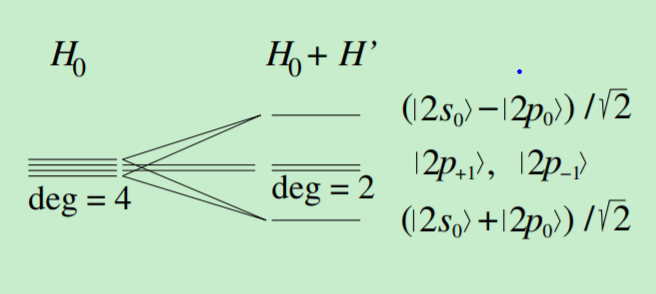
\includegraphics[scale=1]{9_1.PNG}
    \end{minipage}
    \begin{minipage}{0.5\textwidth}
        \captionsetup{font={Large}}
        \caption{Stark effect: the 4-fold degenerate state to n = 2 splits into 2 non-degenerate and a 2-fold degenerate state.}
    \end{minipage}
\end{figure}
We estimate the relative correction,
%公式 58
\begin{equation}
    \frac{e \mathcal{E} a_{0}}{e^{2} / a_{0}}=\frac{\mathcal{E}}{e / a_{0}^{2}}
    \end{equation}
The field $e / a^2_0$ (typical field strength for the $e^−$) is $e / a^2_0 \approx 5 \cdot 109 $V/cm. In addition, the comparison with typical fields in MOSFET’s $\sim 10^5 - 10^6 $V / cm, or the breakthrough field strength of one of the best insulators SiO2 $\sim 10^6 - 10^8 V / cm$. These proportions justify the assumption that the laboratory fields are much smaller than the fields in the atom.

\section{Stationary, almost degenerate case}
Obviously, the series of disturbances is a development in $\langle n|V| l\rangle /\left(\mathcal{E}_{n}-\mathcal{E}_{l}\right)$. If $\mathcal{E}_n\rightarrow\mathcal{E}_l$ goes, the series is only slowly converging. We are discussing the case in which two eigenvectors $| n\rangle$ and $| m\rangle$ degenerate almost (or completely), for example a `level crossing' in the 0 order, cf. figure 9.2.
%图 9.2
\begin{figure}[ht]
    \begin{minipage}{0.5\textwidth}
        \centering
        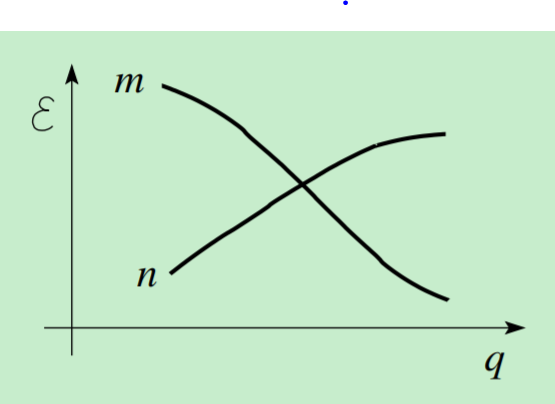
\includegraphics[scale=1]{9_2.PNG}
    \end{minipage}
    \begin{minipage}{0.5\textwidth}
        \captionsetup{font={Large}}
        \caption{`Level Crossing' as a function of the parameter q.}
    \end{minipage}
\end{figure}
We write $H=H_{0}+H^{\prime}=H_{0}+H_{1}^{\prime}+H_{2}^{\prime}$ with
%公式 59
\begin{align} H_{1}^{\prime}=&\left\langle m\left|H^{\prime}\right| m\right\rangle P_{m m}+\left\langle n\left|H^{\prime}\right| n\right\rangle P_{n n} \nonumber\\ &+\left\langle m\left|H^{\prime}\right| n\right\rangle P_{m n}+\left\langle n\left|H^{\prime}\right| m\right\rangle P_{n m} \\ P_{i k}=&|i\rangle\langle k| \end{align}

%公式 60
If $H'_1$ cancels degeneracy in the first order, we can solve $H'_2$ in a conventional manner. The idea is then to first solve the $H_1=H_0+H'_1$ problem exactly and then to treat $H'_2$ perturbatively. Consider $| l\rangle$ with $l \neq m, n.$ With $H_0| l\rangle = \mathcal{E}_l | l\rangle$ also $H_1| l\rangle = \mathcal{E}_l | l\rangle$ since $\langle l | m\rangle = \langle l | n\rangle = 0$ is $\Rightarrow$ nothing to do in $\mathcal{H}\backslash\{\varphi_n,\varphi_m\}$. The $\{\varphi_n,\varphi_m\}$ space remains. But this is precisely the problem (9.33) with

%公式 16
\begin{equation}
\begin{aligned} \mathcal{E}_{m}^{\prime} & \equiv\left\langle m\left|H_{1}\right| m\right\rangle=\mathcal{E}_{m}+\left\langle m\left|H^{\prime}\right| m\right\rangle \\ \mathcal{E}_{n}^{\prime} & \equiv\left\langle n\left|H_{1}\right| n\right\rangle=\mathcal{E}_{n}+\left\langle n\left|H^{\prime}\right| n\right\rangle \\ \delta^{\prime} & \equiv\left\langle m\left|H_{1}\right| n\right\rangle=\left\langle m\left|H^{\prime}\right| n\right\rangle \\ \delta^{\prime *} & \equiv\left\langle n\left|H_{1}\right| m\right\rangle=\left\langle n\left|H^{\prime}\right| m\right\rangle \end{aligned}
\end{equation}
Note that here $\mathcal{E}'_m$ also contains the proportion $\mathcal{E}_m$ in 0th order. In (9.33) $\mathcal{E}_m=\mathcal{E}_n$ and we only considered the perturbation, so we chose the zero point differently. Here  $\mathcal{E}_m\approx\mathcal{E}_n$, but still  $\mathcal{E}_m\neq\mathcal{E}_n$. The new starting vectors and energies for the ¨ $H'_2$ problem are then:
%公式 26
\begin{equation}
\begin{aligned} l \neq m, n &: \mathcal{E}_{l},|l\rangle \\ l=m, n &: \mathcal{E}_{\pm}=\frac{\mathcal{E}_{m}^{\prime}+\mathcal{E}_{n}^{\prime}}{2} \pm \sqrt{\left(\frac{\mathcal{E}_{m}^{\prime}-\mathcal{E}_{n}^{\prime}}{2}\right)^{2}+\left|\delta^{\prime}\right|^{2}} \\ &|\pm\rangle=\frac{1}{\sqrt{2}}\left[\delta^{\prime}|m\rangle+\left(\mathcal{E}_{\pm}-\mathcal{E}_{m}^{\prime}\right)|n\rangle\right] \quad \& \text { standardization. } \end{aligned}
\end{equation}
\textbf{Example: 1D periodic potential.} We consider the problem given by the Hamiltonian $H$ with periodic potential $V (x)$ and periodic (Born-von Karmann) boundary conditions,
%公式 63
\begin{equation}
\begin{aligned} H &=-\frac{\hbar^{2}}{2 m} \partial_{x}^{2}+V(x), \quad V(x+w)=V(x) \\ H \Psi &=E \Psi, \quad \Psi(x+L)=\Psi(x) \end{aligned}
\end{equation}
The undisturbed problem with $H_0 = -\hbar^2\partial_x^2 / 2m$ has the solutions
%公式 64
\begin{equation}
    \varphi_{k}=\frac{1}{\sqrt{L}} e^{i k x}, \quad k=\frac{2 \pi}{L} j, \quad \mathcal{E}_{k}=\frac{\hbar^{2} k^{2}}{2 m}
    \end{equation}
By using periodic boundary conditions, the continuous spectrum is made quasi-continuous ($\rightarrow$ discrete), a suitable technique to handle a continuous spectrum. We want to deal with $V$ theory of theory. With
%公式 65
\begin{equation}
    V(x)=\sum_{l} e^{i K_{l} x} V_{l}, \quad K_{l}=\frac{2 \pi}{w} l
    \end{equation}
(note $V (x + w) = V (x)$ periodically $\Rightarrow V (x)$ can be represented as Fourier series) we obtain for the matrix elements
%公式 66
\begin{equation}
    \left\langle k^{\prime}|V| k\right\rangle=\delta_{k^{\prime}, k+K_{l}} V_{l}
    \end{equation}
and thus find the wave functions in first order perturbation theory
%公式 67
\begin{equation}
    \Psi_{k}(x)=\frac{1}{\sqrt{L}} e^{i k x}+\sum_{l \neq 0} \frac{V_{l}}{\mathcal{E}_{k}-\mathcal{E}_{k+K_{l}}} \frac{1}{\sqrt{L}} e^{i\left(k+K_{l}\right) x}
    \end{equation}
We calculate the energy in 2nd order,

%公式 68
\begin{equation}
    E_{k}=\mathcal{E}_{k}+V_{0}+\sum_{l \neq 0} \frac{\left|V_{l}\right|^{2}}{\mathcal{E}_{k}-\mathcal{E}_{k+K_{l}}}
    \end{equation}
This expression diverges in the vicinity of $\mathcal{E}_{k} \sim \mathcal{E}_{k+K_{l}}$, cf. figure9.3: The $k$ values ​​around $−\pi l / w$ couple via $K_{l}=2 \pi l / w$ to $+\pi l/w$ and the denominators $\mathcal{E}_{k} - \mathcal{E}_{k+K_{l}}$ in (9.68) go towards 0 with $k \rightarrow −l\pi / w$. We therefore solve the problem around $−l\pi / w$ in the context of almost degenerate perturbation theory. With $| m\rangle = \varphi_k$ and $| n\rangle = \varphi_{k + K_l}, k \sim −l\pi / w$, we have the
%图 9.3
\begin{figure}[ht]
        \centering
        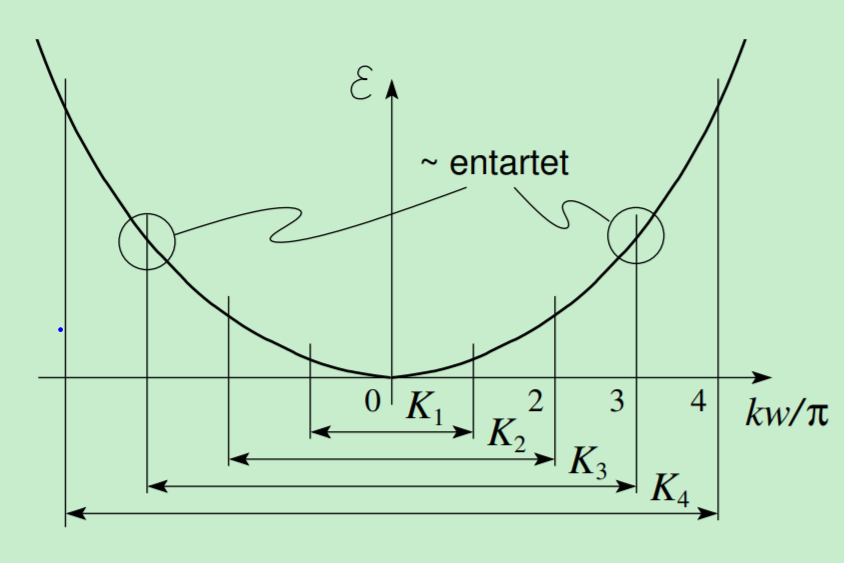
\includegraphics[scale=1]{9_3.PNG}
        \captionsetup{font={Large}}
        \caption{Spectrum of the free solid particle. The states that are symmetrical about the reciprocal lattice vectors $K_l=2\pi l/w$ (with respect to $k = 0$) are degenerate in energy.}
\end{figure}
matrix
%公式 69
\begin{equation}
\left(\begin{array}{cc}{\mathcal{E}_{k}+V_{0}} & {V_{l}^{*}} \\ {V_{l}} & {\mathcal{E}_{k+K_{l}}+V_{0}}\end{array}\right)
\end{equation}
to diagonalize. The energy eigenvalues ​​are

%公式 70
\begin{equation}
    E_{k}^{\pm}=\frac{\mathcal{E}_{k}+\mathcal{E}_{k+K_{l}}}{2}+V_{0} \pm \sqrt{\left(\frac{\mathcal{E}_{k}-\mathcal{E}_{k+K_{l}}}{2}\right)^{2}+\left|V_{l}\right|^{2}}
    \end{equation}
For $\left|\mathcal{E}_{k}-\mathcal{E}_{k+K_{l}}\right| \gg\left|V_{l}\right|$ we get 1-order disorder theory
%公式 17
\begin{equation}
    E_{k}^{+} \approx \mathcal{E}_{k}+V_{0}, \quad E_{k}^{-} \approx \mathcal{E}_{k+K_{l}}+V_{0}
    \end{equation}
At $k = −l\pi / w$ we get substantial corrections,
%公式 27
\begin{equation}
    E_{k}^{+}=\mathcal{E}_{k}+V_{0}+\left|V_{l}\right|, \quad E_{k}^{-}=\mathcal{E}_{k}+V_{0}-\left|V_{l}\right|
    \end{equation}
that is, mixing $k$ and $k + K_l$ creates band gaps in the spectrum. In terms of quality, we get back the spectrum of the Kronig-Penney model, cf. figure 9.4. The band gaps are due to the Fourier coefficients $2 | V_l | = 2 | V (K_l) |$ given, for $V = V_0 \sum\delta (x-lw), V_l = V_0 =$ const.

Usually $| V_l | > | V_{l'} |$ for ¨ $l <l',$ i.e. the gaps decrease with increasing energy; for the ¨ $\delta$-potential (Kronig-Penney model) are the gaps
%图 9.4
\begin{figure}[ht]
    \centering
    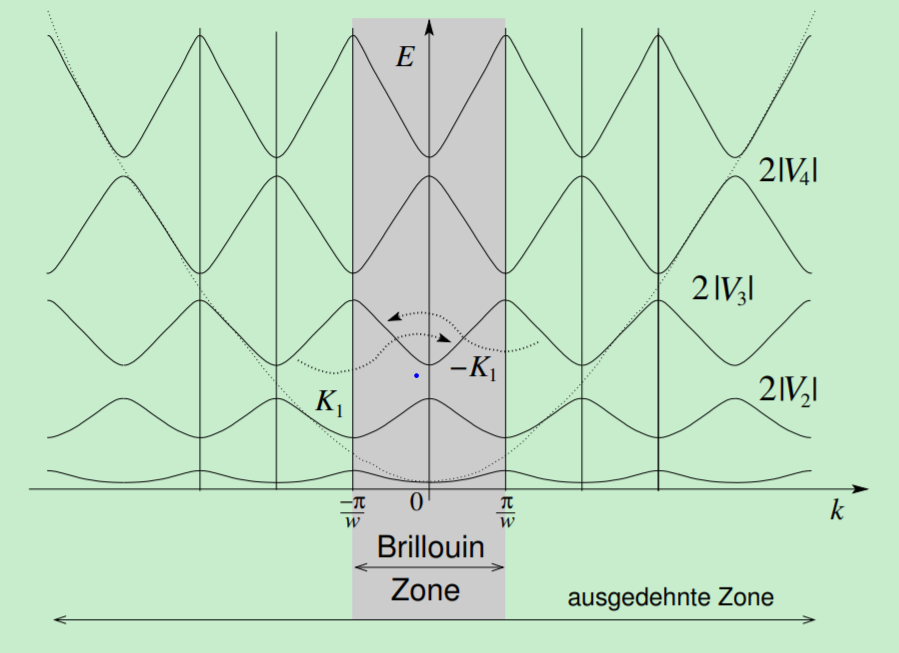
\includegraphics[scale=1]{9_4.PNG}
    \captionsetup{font={Large}}
    \caption{Spectrum of the massive particle in the periodic potential $V (x) = V (x + w)$. The states that are symmetrical about the reciprocal lattice vectors $K_l = 2\pi l/w$ (with reference to $k = 0$) are mixed by the periodic potential and an energy gap of size $2|V_l|$ opens with $V_l$ the Fourier coefficient of the periodic potential. The states in the first Brillouin zone form a complete system; the arrows indicate the shifts in the transition to the reduced band scheme with band indices}
\end{figure}
$2 | V_l | = 2V_0$ maximum. The splitting of the Bloch waves $\Psi_{lk} = exp (ikx) u_l (x)$, cf. (3.81), into a modulation ($exp (ikx)$) and a periodic ($u_l (x)$) part and the accompanying reduction to the first Brillouin zone can easily be done for the extreme case of free electrons (ie, ¨ $V \rightarrow 0$ ) comprehend:
%公式
$$
    \underbrace{
        \begin{array}{ll}
            \Psi_{l k}=e^{i k x} u_{l}(x), & {u_{l}(x)=e^{i K_{l} x}}\\
            &{k \in[-\pi / w, \pi / w]} 
        \end{array}
    }_{\text{reduced}}   
    \hat{=}
    \underbrace{
        \begin{array}{ll}
            \Psi_K &= e^{iKx}.\\
            K &= k+K_l\in\mathbb{R}
        \end{array}
        }_{\text {extended }}
$$
The treatment of the periodic grating in this (fault-theoretical) manner is known as ‘Nearly Free Electron Approximation’ (NFEA). In contrast, the ‘Fast Binding Electron Model’ (Tight Binding Approximation - TBA) starts from bound states, i.e. from localized electrons that bounce with a small amplitude from lattice point to lattice point. With increasing modulation in the potential $V (x)$, the spectrum starts from the steep NFEA form $\sim\hbar^2k^2 / 2m$ with small gaps to the TBA form with flat bands of the form $2t cos (\pi x / w)$ or $2tsin (\pi x / w)$ and large gaps. In this case, $t$ is the matrix element for the hopping electron, i.e. an energy.

\section{Rayleigh-Schrodinger vs. Brillouin Wigner}
In Rayleigh-Schr¨odinger theory, the scheme discussed above, $\Psi$ and $E$ are consistently developed in $\lambda^s$. In contrast, the Brillouin-Wigner theory only develops $\Psi$, but not ¨$ E$, in powers of $H'$. The starting point of the Brillouin-Wigner series of disorders is (9.1),
%公式 73
\begin{equation}
\begin{array}{rcl} 
H \Psi &=&E \Psi \\ & \downarrow&(9.3) \\\left(E-H_{0}\right)|\Psi\rangle &=&\lambda H^{\prime}|\Psi\rangle \\\langle m| \cdot & \downarrow& \\\left(E-\mathcal{E}_{m}\right)\langle m | \Psi\rangle &=&\lambda\left\langle m\left|H^{\prime}\right| \Psi\right\rangle 
\end{array}
\end{equation}
\textbf{Energies:} If we choose $m = n$ and the normalization $\langle n | \Psi\rangle = 1$ we get $\lambda=1$
%
\begin{equation}
    E=\mathcal{E}_{n}+\left\langle n\left|H^{\prime}\right| \Psi\right\rangle
    \end{equation}
identical to (9.12).
States: With | $\Psi$i = Plhl | $\Psi$i | li we immediately get ($\lambda$ = 1)
%公式 75
\begin{equation}
    |\Psi\rangle=|n\rangle+\sum_{l \neq n} \frac{\left\langle l\left|H^{\prime}\right| \Psi\right\rangle}{E-\mathcal{E}_{l}}|l\rangle
    \end{equation}
For comparison, the Rayleigh-Schr¨odinger theory gives the result (see (9.17) - (9.19))
%公式 76
\begin{align}|\Psi\rangle=&|n\rangle+\sum_{l \neq n} \frac{\left\langle l\left|H^{\prime}\right| n\right\rangle}{\mathcal{E}_{n}-\mathcal{E}_{l}}|l\rangle \nonumber\\ &+\sum_{l \neq n}\left(\sum_{k \neq n} \frac{\left\langle l\left|H^{\prime}\right| k\right\rangle\left\langle k\left|H^{\prime}\right| n\right\rangle}{\left(\mathcal{E}_{n}-\mathcal{E}_{l}\right)\left(\mathcal{E}_{n}-\mathcal{E}_{k}\right)}-\frac{\left\langle l\left|H^{\prime}\right| n\right\rangle\left\langle n\left|H^{\prime}\right| n\right\rangle}{\left(\mathcal{E}_{n}-\mathcal{E}_{l}\right)^{2}}\right)|l\rangle \\ &+\cdots \end{align}

%公式 77
On the other hand, the iteration of (9.75)
%公式 78
\begin{equation}
\begin{aligned}|\Psi\rangle=&|n\rangle+\sum_{l \neq n} \frac{\left\langle l\left|H^{\prime}\right| n\right\rangle}{E-\mathcal{E}_{l}}|l\rangle \\ &+\sum_{l \neq n} \sum_{k \neq n} \frac{\left\langle l\left|H^{\prime}\right| k\right\rangle\left\langle k\left|H^{\prime}\right| n\right\rangle}{\left(E-\mathcal{E}_{l}\right)\left(E-\mathcal{E}_{k}\right)}|l\rangle+\cdots \end{aligned}
\end{equation}
Obviously, the series for ¨ | $\Psi$i in the Brillouin-Wigner scheme is much easier to write down. Note, however, that (9.78) on the right contains the unknown energy E. Inserting the perturbation series of E in (9.78) naturally reproduces the Rayleigh-Schr ¨ ¨odinger result (9.76). A remarkable application of (9.78) involves the combination with (9.12), $E = \mathcal{E}_n + \lambda \langle n | H' | \Psi\rangle$, with (9.78) in the s-th approximation, $| \Psi\rangle  \approx | \Psi^{(s)} (E) \rangle$. The solution of the nonlinear equation
%公式 79
\begin{equation}
    E^{(s)}=\mathcal{E}_{n}+\lambda\left\langle n\left|H^{\prime}\right| \Psi^{(s)}(E)\right\rangle
    \end{equation}
by computer a generally very precise determination of $E$ and thus of $\Psi$ in the order $s$ is possible.

\section{Nonstationary perturbation theory}
The non-stationary perturbation theory presents itself with the following typical problem: Given a time-dependent Hamiltonian with the properties
%
\begin{equation}
\begin{aligned} H(t) &=H_{0}+H^{\prime}(t) \\ \partial_{t} H_{0} &=0 \\ H_{0}|n\rangle &=\varepsilon_{n}|n\rangle, \quad|n\rangle \text { ein vONS, } \\ H^{\prime}(t) & \text { time-dependent, small compared } H_{0} \end{aligned}
\end{equation}
The dynamics are defined as follows:
%公式 18
\begin{equation}
\begin{array}{ll}{t<t_{0}:} & {H^{\prime}=0, \quad i \hbar \partial_{t}\left|\Psi^{0}\right\rangle= H_{0}\left|\Psi^{0}\right\rangle} \\ { t>t_{0}:} & {H^{\prime} \neq 0, \quad i \hbar \partial_{t}|\Psi\rangle= H|\Psi\rangle}\end{array}
\end{equation}
with $|\Psi\rangle = | \Psi^0\rangle$ the initial state prepared for ¨ $t <t_0$. We are looking for $|\Psi\rangle$ at times $t> t_0$.

\textbf{Example of a specific question:} Let the system be prepared in an eigenstate of $H_0$ at times $t <t_0$,  $|\Psi^0\rangle=|n\rangle$. With $H'$ = 0 for ¨ $t <t_0$ and  $|\Psi^0\rangle=|n\rangle$, the system develops over time according to $| \Psi^0 (t) \rangle = e^{-i\mathcal{E}_nt/\hbar} | n\rangle$. If we now switch on $H‘$, the $| n\rangle$ are no longer eigenstates of $H$ and are deformed accordingly by the dynamics, ie, $H'$ now mixes other states $l \neq n$ into the time evolution of $| \Psi\rangle\Rightarrow$ Uberg result Changes in other states. We find the amplitudes for these transitions by developing the state disturbed by $H_0$ as a superposition $| \Psi\rangle = \sum_l a_l (t) | l\rangle (\{| l\rangle\}$ is a vONS); the desired transition amplitudes are then given by the ¨ al (t). In Hilbert space the state develops according to sketch 9.5.
%图 9.5
\begin{figure}[ht]
    \begin{minipage}{0.5\textwidth}
        \centering
        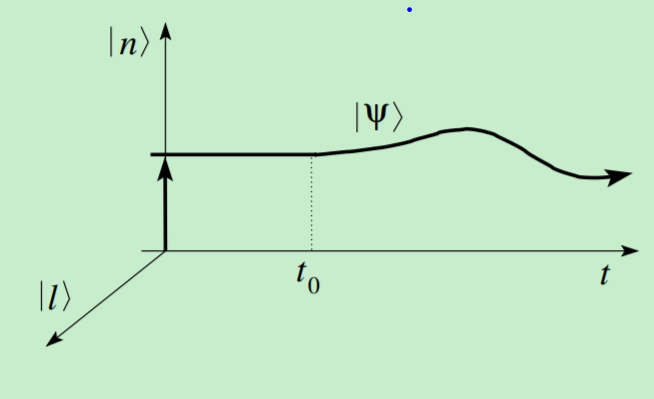
\includegraphics[scale=1]{9_5.PNG}
    \end{minipage}
    \begin{minipage}{0.5\textwidth}
        \captionsetup{font={Large}}
        \caption{If a fault $H'$ is switched on at $t_0$, additional states $|l\rangle$ are added to the eigenstate $|n\rangle$ to $H_0$.}
    \end{minipage}
\end{figure}

\textbf{Solution:} We already derived the adequate formalism in Chapter 7, the interaction picture, see page {\color{red}209}. With
%公式 82
\begin{equation}
    |\Psi(t)\rangle=\underbrace{\exp \left[-i H_{0}\left(t-t_{0}\right) / \hbar\right]}_{U_{0}\left(t, t_{0}\right)}\left|\Psi_{D}(t)\right\rangle
    \end{equation}
and
%公式 83
\begin{equation}
\begin{aligned} \Psi_{D}(t) &=U_{D}\left(t, t_{0}\right) \Psi^{0}\left(t_{0}\right) \\ U_{D}\left(t, t_{0}\right) &=T \exp \left[-\frac{i}{\hbar} \int_{t_{0}}^{t} d t^{\prime} H_{D}^{\prime}\left(t^{\prime}\right)\right] \end{aligned}
\end{equation}
we receive
%公式 84
\begin{equation}
\begin{aligned}|\Psi(t)\rangle=& e^{-i H_{0}\left(t-t_{0}\right) / \hbar}\left[11+\frac{1}{i \hbar} \int_{t_{0}}^{t} d t_{1} H_{D}^{\prime}\left(t_{1}\right)\right.\\ &\left.-\frac{1}{2 \hbar^{2}} \int_{t_{0}}^{t} d t_{1} d t_{2} T\left[H_{D}^{\prime}\left(t_{1}\right) H_{D}^{\prime}\left(t_{2}\right)\right]+\cdots\right]\left|\Psi^{0}\right\rangle \\ H_{D}^{\prime}(t)=& e^{i H_{0}\left(t-t_{0}\right) / \hbar} H^{\prime}(t) e^{-i H_{0}\left(t-t_{0}\right) / \hbar} \end{aligned}
\end{equation}
\subsection{1st order, Fermis Golden Rule}
Consider a system which is prepared for times ¨ $t <t_0$ in the eigenstate $| i\rangle = | $initial$\rangle$ to $H_0$ with energy $\mathcal{E}_i$. What is the probability of finding the system in the state $| f\rangle = | $final$\rangle$ at a later point in time $t> t_0$, where $H_0 | f\rangle = \mathcal{E}_f | f\rangle?$ As an example we call the hydrogen atom in interaction with light (H-atom in the electromagnetic radiation field), whereby the light field acts as a disturbance. In this case, we ask about the transition rates between levels. With ({\color{red}9.84}) we immediately get in first order
%公式 85

\begin{align}\langle f | \Psi\rangle & \cong e^{-i \mathcal{E}_{f}\left(t-t_{0}\right) / \hbar}\left\langle f\left|\mathbb{1}+\frac{1}{i \hbar} \int_{t_{0}}^{t} d t^{\prime} e^{i\left(\mathcal{E}_{f}-\mathcal{E}_{i}\right)\left(t^{\prime}-t_{0}\right) / \hbar} H^{\prime}\left(t^{\prime}\right)\right| i\right\rangle \nonumber\\ & \downarrow\langle f | i\rangle= 0 \nonumber\\ & \cong \frac{1}{i \hbar} \int_{t_{0}}^{t} d t^{\prime}\left\langle f\left|e^{-i \mathcal{E}_{f}\left(t-t^{\prime}\right) / \hbar} H^{\prime}\left(t^{\prime}\right) e^{-i \mathcal{E}_{i}\left(t^{\prime}-t_{0}\right) / \hbar}\right| i\right\rangle \\ 
& \qquad f \quad \stackrel{E_{f}}{\longleftarrow} \quad \stackrel{H'(t')}{\times} \quad \stackrel{\mathcal{E}_{i}}{\longleftarrow} \quad i \end{align}

%公式 86
We get for the transition probability ¨ $P_{i \rightarrow f} (t) = | \langle f | \Psi (t) \rangle |^2$
%公式 78
\begin{equation}
    P_{i \rightarrow f}=\frac{1}{\hbar^{2}}\left|\int_{t_{0}}^{t} d t^{\prime} e^{i\left(\mathcal{E}_{f}-\mathcal{E}_{i}\right) t^{\prime} / \hbar}\left\langle f\left|H^{\prime}\left(t^{\prime}\right)\right| i\right\rangle\right|^{2}
    \end{equation}
To get further we have to make assumptions about the time dependency of the disturbance $H'(t)$. Are common and common cases
\begin{enumerate}
    \item[-] Abrupt turn on: $H'(t) = V\Theta (t - t0)$,
    \item[-] Adiabatic activation from $t <0:$ $H'(t) = V e^{\eta t}, \eta\rightarrow 0^+$, 
    \item[-] Harmonic disturbance: $H'(t) = V \operatorname{cos} wt$. 
\end{enumerate}

We then analyze these three cases.
\begin{enumerate}
    \item[1.] $H' (t) = V \Theta (t - t_0)$
\end{enumerate}
Inserting in (9.87) gives $t_0 = 0$ (oBdA) and the definition $w_{if} = (\mathcal{E}_f - \mathcal{E}_i) / \hbar$
%公式 88
\begin{equation}
\begin{aligned} P_{i \rightarrow f} &=\left|\frac{e^{i \omega_{i f} t}-1}{\hbar \omega_{i f}}\langle f|V| i\rangle\right|^{2} \\ &=\left(\frac{\sin \left(\omega_{i f} t / 2\right)}{\hbar \omega_{i f} / 2}\right)^{2}|\langle f|V| i\rangle|^{2} \end{aligned}
\end{equation}
The factor $\propto \operatorname{sin}^2(w_{if}t/2)$ has zeros at $w_{if}t=2n\pi$ and behaves for $w_{if}\rightarrow 0$ like $(w_{if}t/2)^2/(\hbar w_{if}/2)^2\approx(t/\hbar)^2$, cf. figure 9.6. For long times $t\rightarrow \infty$ we get a sharp peak at $w_{if}=0$ with weight $\propto t$.
%图 9.6
\begin{figure}[ht]
    \begin{minipage}{0.5\textwidth}
        \centering
        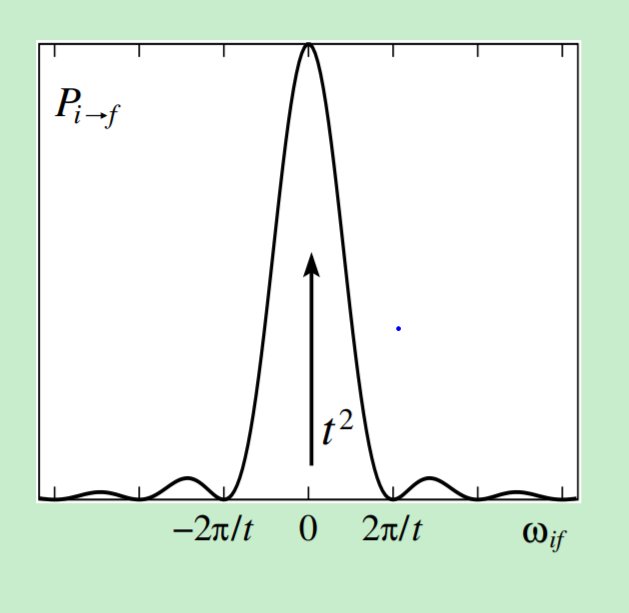
\includegraphics[scale=1]{9_6.PNG}
    \end{minipage}
    \begin{minipage}{0.5\textwidth}
        \captionsetup{font={Large}}
        \caption{Transition amplitude $P_{i \rightarrow f} (w_if)$. The area of the central peak grows according to $t^2\cdot(2\pi/t)\propto t$.}
    \end{minipage}
\end{figure}

\textbf{Interpretation:} After switching on the disturbance, in principle transitions to all energies can take place. The relevant transitions (these are very likely to occur and do not oscillate in time) are those that receive the energy, $w_{if}=0\rightarrow \mathcal{E}_i=\mathcal{E}_f$. The range of energy conservation is given by Heisenberg's unsharp principle,

%公式 89
\begin{equation}
    \Delta \omega_{i f} \cdot t \sim 2 \pi
    \end{equation}
The weight of these energy-conserving processes increases linearly with time,
%公式 90
\begin{equation}
    \int_{2 \pi / t} P_{i \rightarrow f}(\omega) d \omega \sim t
    \end{equation}
For large times higher orders have to be considered. If the spectrum is discrete, it is

%gs91
\begin{equation}
\begin{array}{l}{P_{i \rightarrow f} \sim t^{2} \quad \text { for } \mathcal{E}_{i}=\mathcal{E}_{f}} \\ {P_{i \rightarrow f} \sim \text { oscillates at frequency } \omega_{i f} \text { for } \mathcal{E}_{i} \neq \mathcal{E}_{f}}\end{array}
\end{equation}
In the sequence we consider a continuum of states or a group of final states which are close. The density of these states in the energy space is described by $\rho(\mathcal{E}_f)$, that is, we can replace sums over states $| f\rangle$ by integrals over $\mathcal{E}_f$,

%公式 29
\begin{equation}
    \sum_{f} \rightarrow \int d \mathcal{E}_{f} \rho\left(\mathcal{E}_{f}\right)
    \end{equation}
We further assume that the square of the matrix element $| \langle f | V | i\rangle |^2$ depends on $| f\rangle$ only via $\mathcal{E}_f$.

\textbf{Example:} Free particle in 3D with $E = \hbar^2k^2 / 2m$ and $\vec{k} = 2\pi\vec{n}/ L$ (box normalization to $L^3$). In order to transform the sum into an integral we use the relationship $d^3n = (L / 2\pi)^3d^3k$
%公式 39
\begin{equation}
\begin{array} {rcl}
\sum_{\vec{n}} \rightarrow \frac{L^{3}}{(2 \pi)^{3}} \int d^{3} k&=& \overbrace{L^{3} \int \frac{d \Omega_{k}}{4 \pi}}^{1} k^{2} \frac{d k}{2 \pi^{2}} \\ 
& \downarrow& \rho(k)=L^{3} k^{2} / 2 \pi^{2}, \quad \rho(k) d k=\rho(E) d E \\
& \downarrow &\rho(E)=\rho(k) \cdot \frac{d k}{d E}=L^{3} \frac{2 m E}{2 \pi^{2} \hbar^{2}} \cdot \frac{1}{\hbar} \sqrt{\frac{m}{2 E}} \\ 
& \downarrow &= \frac{mL^3}{2\pi^2\hbar^3}\sqrt{2mE}\\
&=&\int \rho(E) d E \\ 
\Rightarrow \sum_{\vec{n}} &\rightarrow& \int \rho(E) d E \quad \operatorname{with} \rho(E)=\frac{m L^{3}}{2 \pi^{2} \hbar^{3}} \sqrt{2 m E} \end{array}
\end{equation}
Note that $|\langle\vec{k}^{\; \prime}|V|\vec{k}\rangle|^2 $ may only depend on $\vec{k},\vec{k}^{\;\prime}$ via $E_k, E_{k'}$, otherwise $|\langle\vec{k}^{\; \prime}|V|\vec{k}\rangle|^2 $ must be averaged over $\Omega_{\vec{k}\vec{k}^{\;\prime}}$. The above density of states $\rho(E)$ with the volume $L^3$ has the unit $1 / E$. 

The probability of a transition to a state around $|f\rangle$ is then given by

%gs94
\begin{equation}
\begin{aligned} \Gamma t=\sum_{f} P_{i \rightarrow f}(t) &=\int d \mathcal{E}_{f} \rho\left(\mathcal{E}_{f}\right) \frac{\sin ^{2}\left(\omega_{i f} t / 2\right)}{\left(\hbar \omega_{i f} / 2\right)^{2}}|\langle f|V| i\rangle|^{2} \\ &=\left.\frac{2 \pi}{\hbar} t \rho\left(\mathcal{E}_{f}\right)|\langle f|V| i\rangle|^{2}\right|_{\mathcal{E}_{i}=\mathcal{E}_{f}} \end{aligned}
\end{equation}
We have used that $\operatorname{sin}^2(wt)/\pi tw^2\rightarrow\delta(w)$ for $t\rightarrow\infty$, see (2.109); furthermore $d\mathcal{E}_f=\hbar dw_{if}$ and we have assumed that the density of states $\rho(\mathcal{E}_f)$ and the matrix element $|\langle f|V|i\rangle|^2$ are continuous/flat in the vicinity of $\mathcal{E}f$. With this we get for the transition rate $dP_{i\rightarrow f}/dt=\Gamma$,
%gs 95
\begin{equation}
    \Gamma=\frac{2 \pi}{\hbar}|\langle f|V| i\rangle|^{2} \rho\left(\mathcal{E}_{f}\right), \quad \text { Fermi's Golden Rule }
    \end{equation}
with $2\pi\hbar/\Delta\mathcal{E}_f<t\ll 2\pi\hbar/\delta_{\varepsilon}$, cf. figure 9.7. \footnote{Alternatively, you can often find the shape\begin{equation}
    \Gamma=\frac{2 \pi}{\hbar}|\langle f|V| i\rangle|^{2} \delta\left(\mathcal{E}_{f}-\mathcal{E}_{i}\right) \text { Fermi's Golden Rule }
    \end{equation}} The time restrictions have the following origin:
\begin{enumerate}
    \item[-] The peak in $P_{i \rightarrow f}$ must lie within the group of states around $f$. We denote the width of this group with $\Delta\mathcal{E}_f$, especially the matrix element $| \langle i | V | f\rangle |$ approximately constant within $\Delta\mathcal{E}_f$. Then $\Delta\mathcal{E}_f>2\pi\hbar/t$, cf. figure 9.7.
    \item[-] The density under the peak must be sufficiently large, that is, the energy separation $\delta_{\varepsilon}$ between states small, so that many states come to lie within the central peak, $\delta_{\varepsilon}\ll 2\pi\hbar/t$, cf. figure 9.7. 
\end{enumerate}

\textbf{Standardization:} For the scattering of a free particle at the potential ¨$ V$ with amplitude $V_0$ and extension $w \ll\lambda = 2\pi / k$ the matrix element gives $|\langle\vec{k}^{\; \prime}|V|\vec{k}\rangle|^2\sim w^6V_0^2/L^6 $ and the rate results in $\Gamma=mV_0^2w^6\sqrt{2m\varepsilon_f}/\pi\hbar^4L^3$. The volume factor $1 / L^3$ takes account of the  `dilution' of the wave function on the volume $L^3$. If we replace the spreader with $N_d$ independent, randomly distributed defects, the result is the volume-independent result $\Gamma=mV_0^2w^6\sqrt{2m\varepsilon_f}/\pi\hbar^4L^3$ with $ n_d = N_d / L^3$ the defect density.
%公式
\begin{enumerate}
    \item[2.]$
    H^{\prime}(t)=V e^{\eta t}, \quad \eta \rightarrow 0^{+}
$
\end{enumerate}

Inserted in (9.87), this time dependency results in the limit case $t_0\rightarrow -\infty$ fall
%gs 96

%gs97
\begin{equation}
    P_{i \rightarrow f}(t)=\frac{e^{2 \eta t}}{\left(\hbar \omega_{i f}\right)^{2}+(\hbar \eta)^{2}}|\langle f|V| i\rangle|^{2}
    \end{equation}
%图 9.7
\begin{figure}[ht]
        \centering
        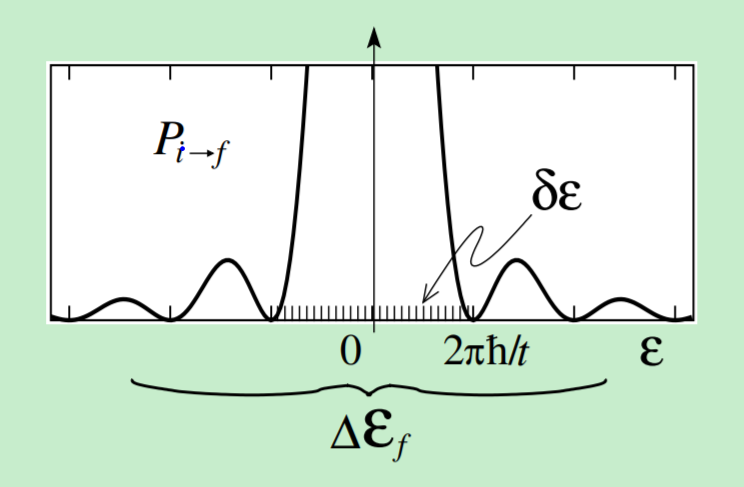
\includegraphics[scale=1]{9_7.PNG}
        \captionsetup{font={Large}}
        \caption{Details on the transition amplitude $P_{i\rightarrow f}(\varepsilon)$. The interval $\Delta\varepsilon_f$ around the final state $| f\rangle$ with matrix elements $| \langle f | V | i\rangle_{\varepsilon_f \in [\Delta \varepsilon_f]} \approx$ const. must be sufficiently wide, $\Delta \varepsilon_f > 2\pi\hbar/t$ (i.e. the matrix element must not change much on the $2\pi\hbar/t$ scale). A small distance between states $\delta_E\ll 2\pi\hbar/t$ (large density of states) guarantees correct ‘sampling’ of the peaks.}
\end{figure}

and we find the transition rate (see again with (¨ 2.109))

%gs98
\begin{equation}
\begin{aligned} \Gamma=\sum_{f} \frac{d}{d t} P_{i \rightarrow f}(t) &=\int d \mathcal{E}_{f} \rho\left(\mathcal{E}_{f}\right) \frac{2 \eta e^{2 \eta t}}{\left(\hbar \omega_{i f}\right)^{2}+(\hbar \eta)^{2}}|\langle f|V| i\rangle|^{2} \\ &=\frac{2 \pi}{\hbar}|\langle f|V| i\rangle|^{2} \rho\left(\mathcal{E}_{f}\right) \end{aligned}
\end{equation}
again in the form of Fermi's Golden Rule.
\begin{enumerate}
    \item[3.] $ H^{\prime}(t)=V \cos \omega t
    $
\end{enumerate}

 We write $H' (t) = V(e^{− iwt} + e^{iwt}) e^{\eta t} / 2$ and choose $t_0\rightarrow-\infty$. Inserting in (9.87) yields (again $\hbar w_{if}=\mathcal{E}_f-\mathcal{E}_i$)
%gs99
\begin{equation}
\begin{aligned} P_{i \rightarrow f}=& \frac{e^{2 \eta t}}{4 \hbar^{2}}|\langle f|V| i\rangle|^{2}\left|\frac{\exp \left[i\left(\omega_{i f}-\omega\right) t\right]}{\omega-\omega_{i f}+i \eta}-\frac{\exp \left[i\left(\omega_{i f}+\omega\right) t\right]}{\omega+\omega_{i f}-i \eta}\right|^{2} \\=& \frac{e^{2 \eta t}}{4 \hbar^{2}}|\langle f|V| i\rangle|^{2}\left[\frac{1}{\left(\omega-\omega_{i f}\right)^{2}+\eta^{2}}+\frac{1}{\left(\omega+\omega_{i f}\right)^{2}+\eta^{2}}\right.\\
&\left.-2 \operatorname{Re} \frac{\exp (-2 i \omega t)}{\left(\omega-\omega_{i f}+i \eta\right)\left(\omega+\omega_{i f}+i \eta\right)}\right] \end{aligned}
\end{equation}
To determine the transition rate $\Gamma$ we calculate the derivative $\partial_t P_{i\rightarrow f}$,
%GS100
{\large{
\begin{equation}
    \begin{aligned}
        \frac{d P_{i \rightarrow f}}{d t}=\frac{e^{2 \eta t}}{4 \hbar^{2}}|\langle f|V| i\rangle|^{2}\left\{\left[\frac{2 \eta}{\left(\omega-\omega_{i f}\right)^{2}+\eta^{2}}+\frac{\frac{2 \pi \delta\left(\omega+\omega_{i f}\right)}{2 \eta}}{\left(\omega+\omega_{i f}\right)^{2}+\eta^{2}}\right](1-\cos 2 \omega t)\right.\\
        \left.+\left[\frac{\omega-\omega_{i f}}{\left(\omega-\omega_{i f}\right)^{2}+\eta^{2}}+\frac{\omega+\omega_{i f}}{\left(\omega+\omega_{i f}\right)^{2}+\eta^{2}}\right](2 \sin 2 \omega t)\right\}
    \end{aligned}
\end{equation}}}
The cos- and sin- proportions average away after a short time. With $\delta(w)/\hbar=\delta(\hbar w)$ we find the result
%公式 101
\begin{equation}
    \Gamma=\frac{2 \pi}{\hbar} \frac{1}{4}|\langle f|V| i\rangle|^{2}\left[\delta\left(\mathcal{E}_{f}-\mathcal{E}_{i}-\hbar \omega\right)+\delta\left(\mathcal{E}_{f}-\mathcal{E}_{i}+\hbar \omega\right)\right]
    \end{equation}
The first term at $\mathcal{E}_f=\mathcal{E}_i+\hbar w$ describes an absorption process, the second term at $\mathcal{E}_f=\mathcal{E}_i-\hbar w$ describes an emission.
\subsection{2nd order}
We choose case 2 with $H'(t) = V e^{\eta t}$ and assume that $\langle f | V | i\rangle = 0$. Then with ({\color{red}9.84})
%公式 102
\begin{equation}
\begin{aligned}\langle f | \Psi\rangle=&-\frac{1}{\hbar^{2}} \int_{-\infty}^{t} d t^{\prime} \int_{-\infty}^{t^{\prime}} d t^{\prime \prime} \\ & \cdot\left\langle f\left|e^{-i H_{0}\left(t-t^{\prime}\right) / \hbar} H^{\prime}\left(t^{\prime}\right) e^{-i H_{0}\left(t^{\prime}-t^{\prime \prime}\right) / \hbar} H^{\prime}\left(t^{\prime \prime}\right) e^{-i H_{0}\left(t^{\prime \prime}-t_{0}\right) / \hbar}\right| i\right\rangle \end{aligned}
\end{equation}
Insertion of $\sum_l|l\rangle\langle l|$, subsequent integration, squaring and derivation after the time $t$ there
%公式 103
\begin{equation}
    \Gamma=\frac{2 \pi}{\hbar}\left|\sum_{l} \frac{\langle f|V| l\rangle\langle l|V| i\rangle}{\mathcal{E}_{i}-\mathcal{E}_{l}+i \eta \hbar}\right|^{2} \delta\left(\mathcal{E}_{f}-\mathcal{E}_{i}\right)
    \end{equation}
the result is a limit $\eta\rightarrow 0^+$. The rate involves the second order matrix element $|\sum\mathop{-}\limits_{\cdots}^{...}|^2$  with transitions $| i\rangle\rightarrow | f\rangle$ via $| l\rangle$,
%公式 104
\begin{equation}
    |i\rangle \longrightarrow|l\rangle \longrightarrow|f\rangle
    \end{equation}
\subsection{decay of a state}
To determine the decay rate of the state $| i\rangle$ we calculate $\langle f | \Psi\rangle$ with $\langle f | = \langle i |$. It is
%公式 105
\begin{equation}
\begin{aligned}\langle i | \Psi\rangle &= e^{-i \mathcal{E}_{i}\left(t-t_{0}\right) / \hbar}\left\langle i | \Psi_{D}\right\rangle \\ i \hbar \partial_{t}\left|\Psi_{D}\right\rangle &= H_{D}^{\prime}(t)\left|\Psi_{D}\right\rangle \end{aligned}
\end{equation}
We take the matrix element with $\langle i |$ and divide by $\langle i | \Psi_D\rangle$,
%公式 106
\begin{equation}
    i \hbar \partial_{t} \ln \left\langle i | \Psi_{D}\right\rangle=\left\langle i\left|H_{D}^{\prime}(t)\right| i\right\rangle+\sum_{l \neq i}\left\langle i\left|H_{D}^{\prime}(t)\right| l\right\rangle \frac{\left\langle l | \Psi_{D}\right\rangle}{\left\langle i | \Psi_{D}\right\rangle}
    \end{equation}
We can write in order $H'^{\;2}$ (cf. (9.85); development up to the 1st order is sufficient)
%公式 107
\begin{equation}
    \left\langle l | \Psi_{D}\right\rangle \approx \frac{1}{i \hbar} \int_{t_{0}}^{t} d t^{\prime}\left\langle l\left|H_{D}^{\prime}\left(t^{\prime}\right)\right| i\right\rangle
    \end{equation}
and with $\langle i | \Psi_D\rangle\approx \langle i | i\rangle = 1$ we find

%公式 108
\begin{equation}
\begin{aligned} i \hbar \partial_{t} \ln \left\langle i | \Psi_{D}\right\rangle &=\left\langle i\left|H_{D}^{\prime}(t)\right| i\right\rangle+\sum_{l \neq i} \frac{1}{i \hbar} \int_{t_{0}}^{t} d t^{\prime}\left\langle i\left|H_{D}^{\prime}(t)\right| l\right\rangle\left\langle l\left|H_{D}^{\prime}\left(t^{\prime}\right)\right| i\right\rangle \\ & \downarrow H^{\prime}=e^{\eta t} V, \text { mit } \eta \rightarrow 0^{+} \\ &=\langle i|V| i\rangle+\sum_{l \neq i} \frac{|\langle i|V| l\rangle|^{2}}{\mathcal{E}_{i}-\mathcal{E}_{l}+i \eta \hbar} \end{aligned}
\end{equation}
\textbf{Discrete spectrum:} With $\eta\rightarrow 0^+$ we find
%公式 109
\begin{equation}
\begin{array}{rcl} i \hbar \partial_{t} \ln \left\langle i | \Psi_{D}\right\rangle &\stackrel{(9.17)-(9.19)}{=}& E_{1}+E_{2} \\ i \hbar \partial_{t} \ln \langle i | \Psi\rangle &=&\varepsilon_{i}+E_{1}+E_{2}=E_{i}^{(2)} \end{array}
\end{equation}
that is, we are just finding the time evolution which is given by the energy $E^{(2)}_i$ of the state corrected in 2nd order. Interpretation: The discrete state $| i\rangle$ is adiabatically deformed by $H'$, as shown in figure 9.8.

\textbf{Continuum:} There is $| i\rangle$ in a continuum of states. The divergence at 0 produced by the energy denominator $\mathcal{E}_i-\mathcal{E}_l+i\eta\hbar$ is dealt with in the distributive sense as given by the theory of functions, cf. figure 9.9, using Sokhotski's formula
%图 9.8
\begin{figure}[ht]
    \begin{minipage}{0.6\textwidth}
        \centering
        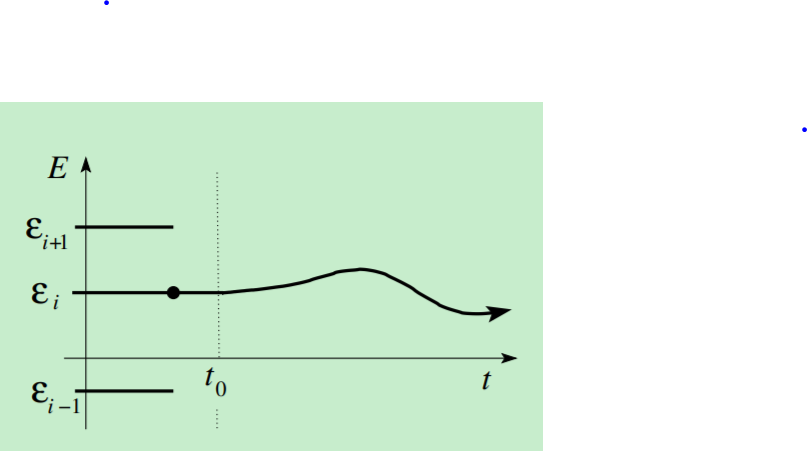
\includegraphics[scale=1.4]{9_8.PNG}
    \end{minipage}
    \begin{minipage}{0.4\textwidth}
        \captionsetup{font={Large}}
        \caption{Adiabatic Deformation: The discrete state $| i\rangle$ is only deformed by the disturbance $H'$; there are no transitions to other states.}
    \end{minipage}
\end{figure}

%公式 110
\begin{equation}
    \int d x \frac{f(x)}{x \pm i \varepsilon}=\int_{-\infty}^{-\varepsilon}+\int_{\varepsilon}^{\infty} d x \frac{f(x)}{x} \mp i \pi f(0)
    \end{equation}
with the interval $[−\mathcal{E}, \mathcal{E}]$ being excluded in the integral (main value). That's how we get

%公式 111
\begin{equation}
\begin{aligned} i \hbar \partial_{t} \ln \langle i | \Psi\rangle=& \underbrace{\mathcal{E}_{i}+\langle i|V| i\rangle+ f d \mathcal{E}_{l} \rho\left(\mathcal{E}_{l}\right) \frac{|\langle i|V| l\rangle|^{2}}{\mathcal{E}_{i}-\mathcal{E}_{l}}}_{E_{i}^{(2)}} \\ &-\underbrace{i \pi \int d \mathcal{E}_{l} \rho\left(\mathcal{E}_{l}\right)|\langle i|V| l\rangle|^{2} \delta\left(\mathcal{E}_{i}-\mathcal{E}_{l}\right)}_{\hbar \Gamma / 2} \end{aligned}
\end{equation}
%图 9.9
\begin{figure}[ht]
    \begin{minipage}{0.5\textwidth}
        \centering
        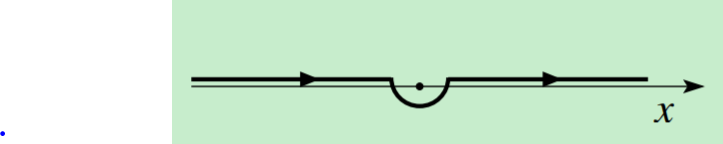
\includegraphics[scale=1]{9_9.PNG}
    \end{minipage}
    \begin{minipage}{0.5\textwidth}
        \captionsetup{font={Large}}
        \caption{Regularization of a pole $[x − i\varepsilon] ^{−1}$ using Sokhotski's formula.}
    \end{minipage}
\end{figure}
The time evolution of $\langle i | \Psi\rangle$ is then given by
%公式 112
\begin{equation}
    \langle i | \Psi\rangle \sim e^{-i E_{i}^{(2)} t / \hbar} e^{-\Gamma t / 2}=e^{-i E t / \hbar}
    \end{equation}
with $E = E^{(2)}_i -i\Gamma / 2$. The Fourier transformation in time (with $\operatorname{exp}^{(-iwt)})$ produces a $\delta$-function $\delta(\hbar w-E)$ for a stationary state with energy $E$, that is, the energy is sharp. By contrast, the decaying state (9.112) is described by a pole in the lower complex half-plane - the energy is not sharp, the state decays with a half-life of $1 / \Gamma$, cf. figure 9.10. Interesting problems arise when two levels meet as a function of the parameter $\alpha(t)$, cf. Figure 9.11. Usually produced
\begin{figure}[ht]
    \begin{minipage}{0.5\textwidth}
        \centering
        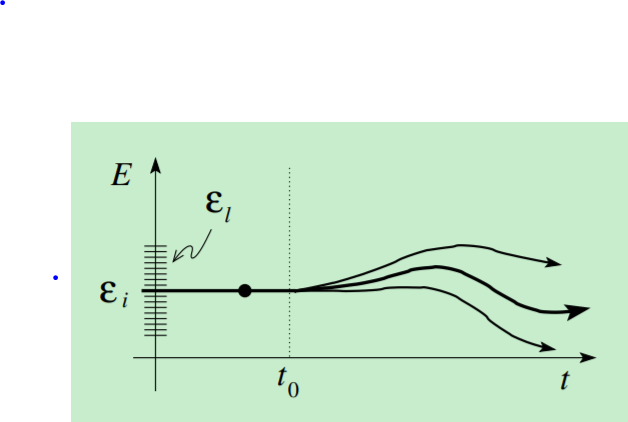
\includegraphics[scale=1]{9_10.PNG}
    \end{minipage}
    \begin{minipage}{0.5\textwidth}
        \captionsetup{font={Large}}
        \caption{Decay of the state $| i\rangle$ in the continuum due to a disturbance $H'$.}
    \end{minipage}
\end{figure}
a mixed term in Hamiltonian a repulsion between the levels (avoided level crossing). Depending on how fast the parameter $\alpha$ changes over time, one finds that the state $| i\rangle$ follows its energy level (adiabatic limit) or else jumps to the next state (diabatic limit). The associated keyword is  `Landau-Zener' tunnels, which tunnel through a forbidden zone between energy levels.
%图 9.11
\begin{figure}[ht]
        \centering
        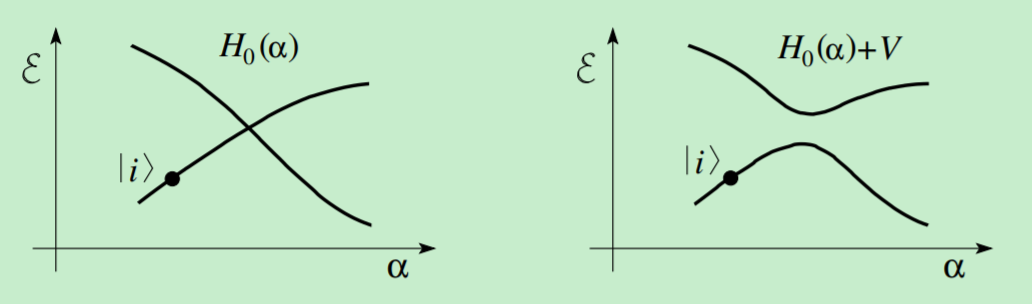
\includegraphics[scale=1.5]{9_11.PNG}
        \captionsetup{font={Large}}
        \caption{Two intersecting states (different symmetry, left) are mixed by a symmetry-breaking disturbance $V$, which creates an energy gap in the spectrum. The state ¨ $| i\rangle$ is deformed by the parameter α. If $\alpha$ is changed quickly, $| i\rangle$ follows the original level of the same symmetry and jumps over the gaps (Landau-Zener tunnels). If $\alpha$ is changed slowly, $| i\rangle$ follows the new ground state.}
\end{figure}